%!TEX root = ../../report.tex
\chapter{Overall Design Principles} % (fold)
\label{chap:overall_design_principles}
The goal of catching a ball is realised using a combination of analogue and digital circuitry, firmware for a soft microprocessor and a PC program featuring a GUI to visualise the impact point of the ball.
Digital logic and a MicroBlaze soft microprocessor is described in VHDL and implemented on a Xilinx Spartan-3E FPGA, firmware is written in C and the GUI program is written in C++ using the Qt framework.
A physical platform and arm is built to mount the electronics on and enable actuation of a arm with a basket to catch a ball.
%
	\section{Components overview}
	Figure \ref{fig:overview} depicts an overview diagram of the components used in the combined system and how they interface with each other.
	The current produced by the piezoelectric sensors is used to pull FPGA pins to a voltage level which represents logic high.
	\begin{figure}[htb]
		\centering
		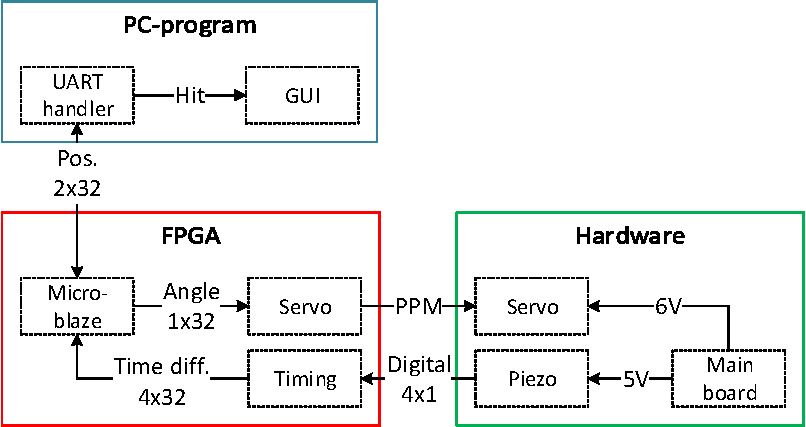
\includegraphics[width=1\textwidth]{figures/overview}
		\caption{Top level diagram of the combined system components with bus widths assigned.}
		\label{fig:overview}
	\end{figure}
	%
	Once a piezoelectric sensor triggers an input pin on the FPGA, the current system time is noted.
	When all four inputs have been triggered, the microprocessor receives an interrupt and begins finding the $(x,y)$-position of the impact point.
	The solution is used to actuate the arm and position it to catch the ball as it returns to the platform after the first bounce.
	
	The impact point is stored in microprocessor memory until the next ball-impact, and can be requested by the PC program through UART.
	Finally the GUI shows a visual interpretation of the data. The determination of the impact point is determined by solving the time difference of arrival problem(TDOA).
	%
	\section{Time difference of arrival}
	In this section the relationship between differences in time measurements from multiple sensors and the $(x,y)$-position of the emitter are derived.
	The problem can be modelled as in figure \ref{fig:tdoa_model} where the following parameters are constants given from the physical configuration and measurements:
	\begin{itemize}
		\item Time of arrival of sound at sensors $a$, $b$, $c$ and $d$.
		\item Speed of sound in chosen material.
		\item Position of sensors.
	\end{itemize}

	The system is set up with four sensors because the risk of obtaining multiple solutions when using only three \cite{tdoa_book}.
	The solution will be represented as a system of linear equations to enable fast and relatively simple implementation in C.
	The derivation will be conducted for two of the sensors, giving one row in the system of equations. The remaining two rows are determined in a similar manner.
	\begin{figure}[htb]
		\centering
		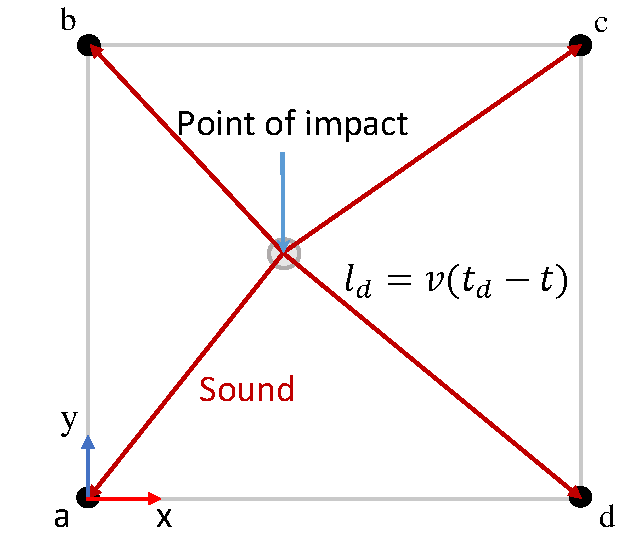
\includegraphics[width=.6\textwidth]{figures/tdoa_model}
		\caption{Top-down view of platform surface area showing sensors and impact point.}
		\label{fig:tdoa_model}
	\end{figure}
	%
	Assuming constant speed of sound through the impact plane, \eqref{eq:speedOfSoundDistA} describes the relationship between time difference between measurement and impact $(t_a - t)$ and the distance the impact point is from sensor $a$.
	\begin{equation}
		l_a = v(t_a - t) \Leftrightarrow l_a^2 = v^2(t_a - t)^2
		\label{eq:speedOfSoundDistA}
	\end{equation}
	Eq. \ref{eq:speedOfSoundDistB} describes the same relationship with respect to sensor $b$.
	\begin{equation}
		l_b = v(t_b - t) \Leftrightarrow l_b^2 = v^2(t_b - t)^2
	\label{eq:speedOfSoundDistB}
	\end{equation}
	By differencing \eqref{eq:speedOfSoundDistA} and \eqref{eq:speedOfSoundDistB}, \eqref{eq:distanceDiffRelativeToTime} can be derived using the difference of squares formula. It is a linear relation with respect to time of impact $t$.
	\begin{equation}
		l_a^2 - l_b^2 = v^2(t_a^2 - t_b^2) - 2 v^2 (t_a - t_b) t
		\label{eq:distanceDiffRelativeToTime}
	\end{equation}
	By using Pythagoras theorem the difference in squared distances from the impact point are also related according to \eqref{eq:distDifference}. It can be seen that it is a linear equation in x and y with constants given from the setup.
	\begin{equation}
		\begin{split}
			l_a^2 - l_b^2 & = (x_a - x_b)^2 + (y_a - y)^2 - ((x_b-x)+(-y_b - y))^2 \\
			& = -2( (x_a - x_b) x + (y_a - y_b) y ) + x_a^2 +y_a^2 -(x_b^2 + y_b^2)
		\end{split}
		\label{eq:distDifference}
	\end{equation}
	By setting \eqref{eq:distanceDiffRelativeToTime} and \eqref{eq:distDifference} equal and isolating the constants known from time measurements and setup, \eqref{eq:firstRow} is derived.
	\begin{equation}
		(x_a - x_b) x + (y_a - y_b) y - v^2(t_a - t_b) t = (x_a^2 +y_a^2 -(x_b^2 + y_b^2) - v^2(t_a^2 - t_b^2))/2 \equiv k_{ab}
		\label{eq:firstRow}
	\end{equation}
	Using similar relations for the other four sensors results in the system of linear equations \eqref{eq:linsys} which solution uniquely defines the $(x,y)$-position of the impact point \cite{tdoa_notes}.
	\begin{equation}
		\begin{bmatrix}
			x_a - x_b & y_a - y_b & - v^2(t_a - t_b) \\
			x_b - x_c & y_b - y_c & - v^2(t_b - t_c) \\
			x_c - x_d & y_c - y_d & - v^2(t_c - t_d)
		 \end{bmatrix}
		 \left[ \begin{array}{c} x \\ y \\ t \end{array} \right] = \left[ \begin{array}{c} k_{ab} \\ k_{bc} \\ k_{cd}\end{array} \right]
		 \label{eq:linsys}
	\end{equation}
% chapter overall_design_priciples (end)